
\section{Designing SimpleSpeech}

Building on the capabilities developed in these prior studies, SimpleSpeech is a web-based application for recording and editing short voice messages in a discussion setting (see Fig. \ref{fig:overview_shot}).
The design of SimpleSpeech is inspired by the transcription-based speech editing systems developed by Rubin \cite{rubin}, Yoon \cite{yoon}, and Whittaker \cite{whittaker_semantic}, which also use ASR transcription as a semantic and visual proxy for audio.
Conceptual modifications were necessary to suit the ``live'' editing paradigm, in which the user records and edits spoken comments in a unified workflow.

We followed an iterative procedure to improve the design and interactions of SimpleSpeech.
After building an initial prototype of the application, an informal pilot test was conducted with 5 participants. 
Each user was given a brief introduction to the software and shown how to use the basic features, then given the scenario of creating an audio response to a written claim on an online forum. 
The prompts used in the tests were adapted from the GRE Pool of Issue Topics.
This user feedback helped us improve the capabilities of SimpleSpeech in several ways:

\begin{itemize}
	\item \emph{Pause manipulation}. An important finding in the pilot study was the importance of being able to introduce and adjust pauses between words, not just to remove them.
	These gaps in the audio help make natural-sounding cuts between audio clips as well as to punctuate claims (e.g., the end of a sentence). 
	The original system only allowed the user to delete pauses, so we added a spacebar action to insert a fragment of silence.
	\item \emph{Live insertion}. Users often misspoke a word or phrase in the middle of a message.
	Since re-recording the entire message was a large burden, a partial deletion and re-recording capability was required.
	Our interface maintains the text-based principle that the cursor position uniformly indicates the focus of editing.
	Therefore, in SimpleSpeech, clicking the Record button naturally inserts a new stream into the existing audio at the point corresponding to the cursor position.
	\item \emph{Quasi-modal transcription editing}. In consideration of the recipient, the pilot testers wanted to correct ASR errors.
	We found that an interface with an audio-editing mode for revising speech and a text-editing mode for correcting mistranscriptions confused users.
	This led us to design a small, separate quasi-modal editing box (see Fig. \ref{fig:transcription}) that pops up during transcription editing.
	The movement of the cursor to the modal box clearly indicates that the system is in a separate text-editing mode, accessed by pressing the Return key.
\end{itemize}



\begin{figure}
	\centering
	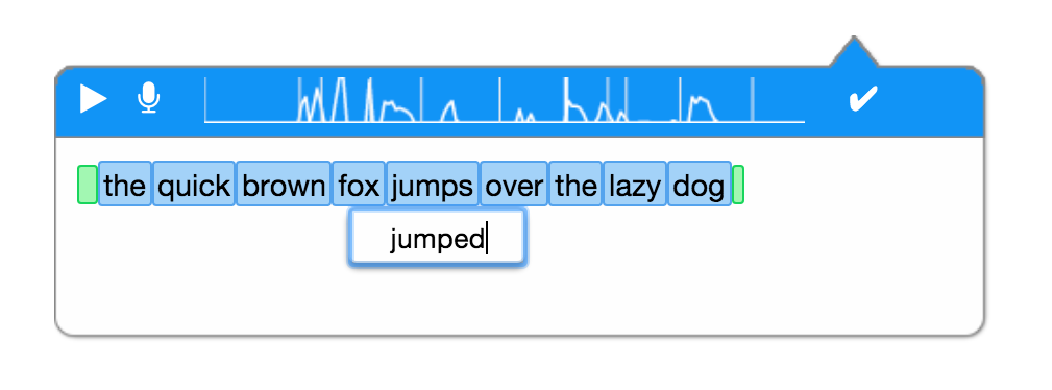
\includegraphics[width=\columnwidth,keepaspectratio]{figures/transcription_edit}
	\caption{To keep the user interface from becoming cluttered with secondary functionality, the transcription editing feature was implemented as a modal interaction. The pop-up box shown above gives clear visual indication to the user that they are no longer directly editing the audio.}
	\label{fig:transcription}
\end{figure}


Our text-based approach to speech editing requires a reliable transcription as well as time intervals corresponding to each word.
Both of these requirements are fulfilled by the IBM Watson Developer Cloud speech-to-text transcription service, which is reported to have a word error rate of around 10\% \cite{soltau:2014}.
